\documentclass[10pt]{article}
% Math Packages
\usepackage{amsmath, mathtools}
\usepackage{amssymb}
\usepackage{amsthm}
\usepackage{amsfonts}
\usepackage{bbm}
\usepackage{breqn}
\usepackage[margin=1in]{geometry}
\usepackage{graphicx}
\usepackage{tikz}
\usetikzlibrary{arrows.meta}
\usetikzlibrary{calc}
\usepackage{forest}
\usepackage{tikz-qtree}
\graphicspath{ {./images/} }
\usepackage{hyperref}
\usepackage[capitalize]{cleveref}
\usepackage[shortlabels]{enumitem}
\usetikzlibrary{arrows,matrix,positioning}
\usepackage{multicol}


\usepackage{empheq} % for boxed equations
\usepackage[most]{tcolorbox}
\newtcbox{\mymath}[1][]{%
  nobeforeafter, math upper, tcbox raise base,
  enhanced, colframe=blue!30!black,
  colback=blue!30, boxrule=1pt,
  #1}
\newtcbox{\boxmath}[1][]{%
  nobeforeafter, math upper, tcbox raise base,
  enhanced, colframe=blue!30!black,
  boxrule=1pt,
  #1}



% for the pipe symbol
\usepackage[T1]{fontenc}

% color
\usepackage{xcolor} 
\definecolor{RoyalBlue}{cmyk}{1, 0.50, 0, 0}
\definecolor{Red}{rgb}{1,0,0}
\definecolor{Blue}{rgb}{0,0,1}
\definecolor{Purple}{rgb}{.75,0,.25}
\newcommand{\rnote}[1]{\textcolor{Red}{[#1]}}       % Red note
\newcommand{\pnote}[1]{\textcolor{Purple}{[#1]}}    % Purple note
\newcommand{\bnote}[1]{\textcolor{Blue}{#1}}        % Blue text
\newcommand{\Max}[1]{\pnote{#1}}                    % Alias for purple note
\DeclareRobustCommand{\demph}[1]{% definitions
  \ifmmode
  {\color{Blue}#1}%
  \else
  {\color{Blue}\bfseries\slshape #1}%
  \fi
}
% \newcommand{\demph}[1]{\textcolor{RoyalBlue}{\textbf{\slshape #1}}} % Slanted RoyalBlue text
\def\red{\color{Red}} \def\blue{\color{Blue}}
\def\gray{\color{gray}} \def\purple{\color{Purple}}

% Claim numbering (the counter restarts after each proof environment)
\newcounter{claimcount}
\setcounter{claimcount}{0}
\newenvironment{claim}{\refstepcounter{claimcount}\par\addvspace{\medskipamount}\noindent\textbf{Claim \arabic{claimcount}:}}{}
\usepackage{etoolbox}
\AtBeginEnvironment{proof}{\setcounter{claimcount}{0}}
\newenvironment{claimproof}{\par\addvspace{\medskipamount}\noindent\textit{Proof of Claim  \arabic{claimcount}.}}{\hfill\ensuremath{\qedsymbol} \tiny{Claim}

  \medskip}
% Add claim support to cleverref
\crefname{claimcount}{Claim}{Claims}

\usepackage[most]{tcolorbox} % for boxed text,
% use \begin{tcolorbox[width=0.7\linewidth,
%   colback=white, colframe=black]}

% Math Environments
\newtheorem{theorem}{Theorem}
\newtheorem{assumption}[theorem]{Assumption}
\newtheorem{lemma}[theorem]{Lemma}
\newtheorem{proposition}[theorem]{Proposition}
\newtheorem{corollary}[theorem]{Corollary}
\newtheorem{question}[theorem]{Question}
\newtheorem{remark}[theorem]{Remark}
\theoremstyle{definition}
\newtheorem{definition}[theorem]{Definition}
\newtheorem{example}[theorem]{Example}
\newtheorem{notation}[theorem]{Notation}
\newtheorem{problem}[theorem]{Problem}


% Redefine the Example environment to include "End of example [number]"
\makeatletter
\let\oldexample\example
\renewenvironment{example}
{\begin{oldexample}}
  {\par\smallskip\hfill   End of Example~\theexample. $\square$    \par\end{oldexample}}
\makeatother

% Redefine the Remark environment to include "End of remark [number]"
\makeatletter
\let\oldremark\remark
\renewenvironment{remark}
{\begin{oldremark}} 
  {\par\smallskip\hfill   End of Remark~\theremark. $\square$    \par\end{oldremark}}
\makeatother


\usepackage{skull}


% Custom Math Coqmmands
\newcommand{\vt}{\vskip 5mm} % vertical space
\newcommand{\fl}{\noindent\textbf} % first line
\newcommand{\Fl}{\vt\noindent\textbf} % first line with space above
\newcommand{\Fli}{\vskip 2mm\noindent\textit} % first line with space above
\newcommand{\norm}[1]{\left\lVert#1\right\rVert} % norm
\newcommand{\1}[1]{\textbf{1}_{\left[#1\right]}} % indicator function 
\def\limn{\lim_{n\to\infty}} % shortcut for lim as n-> infinity
\def\sumn{\sum_{n=1}^{\infty}} % shortcut for sum from n=1 to infinity
\def\sumkn{\sum_{k=1}^{n}} % shortcut for sum from k=1 to n
\def\sumin{\sum_{i=1}^{n}} % shortcut for sum from i=1 to n
\def\R{\mathbb{R}} % Real numbers
\def\N{\mathbb{N}} % Natural numbers
\def\Z{\mathbb{Z}} % Integers
\def\Q{\mathbb{Q}} % Q probability
\def\dist{\text{dist}} %Text 'dist' for things like 'dist(x,y)'

% Brackets and Parentheses
\def\[{\left [}
    \def\]{\right ]}




\title{Lecture Notes for Math 243: \\ Calculus III}
\date{Last updated: \today}
% \author{mh}

\begin{document}
\maketitle
\tableofcontents
\newpage
% \section*{About this document}

% These lecture notes were prepared by Max Hill for a 16-week Calculus III course  (MATH
% 243) at University of Hawaii at Manoa in Spring 2025. This course emphasizes differentiation, as UH Manoa
% has a Calclulus IV devoted to integration theory.

% The textbook used is James Stewart's \textit{Calculus} (8th edition), in which we cover primarily
% chapters 10, 12, 13, and 14. In addition to this text, the material in these lecture notes is also based
% on a number of other sources as well, including:
% \begin{itemize}
%   \item Stephen Abbott's \textit{Understanding Analysis} (2001) 
%   \item Gilbert Strang's \textit{Calculus}, freely available at
%   \url{https://ocw.mit.edu/ans7870/resources/Strang/Edited/Calculus/Calculus.pdf}
%   \item \textit{Supplementary Notes for Calculus II}, written by Michael Olinick
%   with the assistance of John D. Emerson. These are course notes for a calculus
%   class from 2012.
%   \item Sigurd B. Angenent's \textit{Math 222 - 2nd Semester Calculus} lecture
%   notes (2013)
%   \url{https://people.math.wisc.edu/~angenent/222.2013s/UWMath222_2013s.pdf}
%   \item Steve Butler's calculus notes available at
%   \url{https://www.calc2.org/previous-examsquizzes}
%   \item Michael Fowler's text at
%   \url{https://galileoandeinstein.phys.virginia.edu/lectures/momentum.html}, for physics stuff
% \end{itemize}
% Most of the figures were produced with ChatGPT using the tikz package.

\newpage
\setcounter{section}{-1}
\section{Tentative Course Outline}


\begin{itemize}
  \item \textbf{Weeks 1-3:} Parametric equations and Polar coordinates
  \begin{enumerate}
    \item Arc length
    \item Curves defined by parametric equations.
    \item Calculus with plane curves.
    \item Polar coordinates
    \item Areas and lengths in polar coordinates
    \item Conic sections.
  \end{enumerate}
  \item \textbf{Weeks 4-6:} Vectors and the geometry of space.
  \begin{enumerate}
    \item Three-dimensional coordinate systems.
    \item Vectors.
    \item The dot product.
    \item The cross product.
    \item Equations of lines and planes.
    \item Cylinders and quadric surfaces.
  \end{enumerate}
  \item \textbf{Friday, October 16 (week 8):} Midterm exam

  \item \textbf{Weeks 7-9:} Vector functions.
  \begin{enumerate}
    \item Vector functions and space curves
    \item Derivatives and integrals of vector functions.
    \item Arc length and curvature.
    \item Motion in space: velocity and acceleration.
  \end{enumerate}
  \item \textbf{Weeks 10-16:} Partial derivatives.
  \begin{enumerate}
    \item Functions of several variables.
    \item Limits and continuity
    \item Partial derivatives.
    \item Tangent planes and linear approximations
    \item The chain rule.
    \item Directional derivatives and the gradient vector.
    \item Maximum and minimum values.
    \item Discovery project (p.1010 Stewart): Quadratic approximation and critical
    points (Taylor’s formula for two variables).
    \item Lagrange multipliers.
  \end{enumerate}
  \item \textbf{Monday, December 14:} Final exam.
\end{itemize} 

\newpage
\section{2026-08-24 | Week 01 | Lecture 01}
\textit{This lecture is based on textbook section 6.3. ``Arc length''}

\begin{center}
  \begin{tcolorbox}[width=0.9\textwidth, colback=white, colframe=black]
    \textit{\textbf{The nexus question of this lecture:} How do we compute the
      length of a curve, assuming the curve is the graph of a function?}
  \end{tcolorbox}
\end{center}

\subsection{Arc Length}


First, recall the definition of \demph{derivative}:
\begin{align*}
  f'(x) 
  &:= \lim_{h\to 0}\frac{f(x+h)-f(x)}{h}\\
\end{align*}
or equivalently,
\begin{equation*}
  f'(x) = \lim_{\tilde{x} \to x} \frac{f(\tilde{x})-f(x)}{\tilde{x}-x}
\end{equation*}
In other words, the derivative is obtained by computing 
\begin{equation*}
  \frac{\text{change in $y$-value}}{\text{change in $x$-value}}  = \frac{\Delta y}{\Delta x}
\end{equation*}
as $\Delta x \to  0$.


One of the central ideas in calculus is to approximate curvy things with flat things. For example, if
faced with a curve, approximate it with straight lines. For example,


\fl{Problem:} I am an ant, and I want to travel from $a$ to $b$ by walking on the graph of
$f(x)$. How far must I walk?

\fl{Strategy:} Cheat a little: think of the ant walking in a bunch of straight lines that are pretty
close to the curve.

\begin{center}
  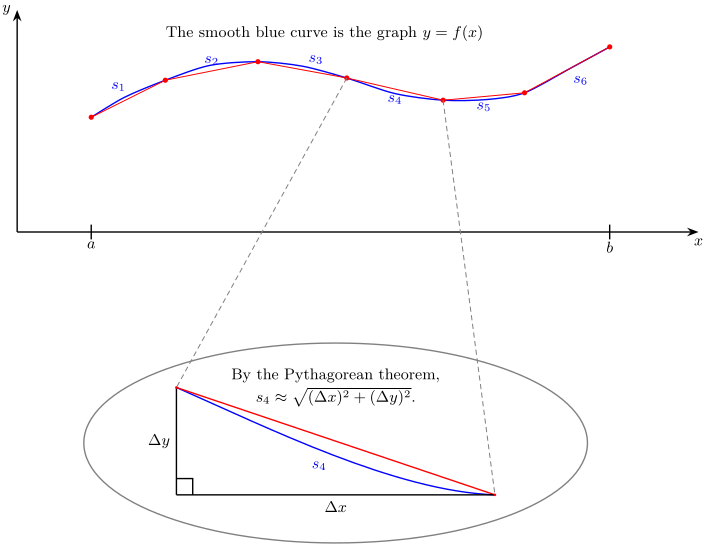
\includegraphics[scale =.5]{images/arc-length-justification-tikz}
\end{center}

% \usetikzlibrary{arrows.meta,calc}

% \begin{tikzpicture}[
%   scale=1.5,
%   >=Stealth,
%   axis/.style={->, thick},
%   curve/.style={blue, thick},
%   secant/.style={red},
%   guide/.style={densely dashed, gray},
%   every node/.style={font=\small}
%   ]

%   % Axes
%   \draw[axis] (0,0) -- (9.2,0) node[below] {$x$};
%   \draw[axis] (0,0) -- (0,3) node[left] {$y$};

%   % Endpoints of the interval
%   \coordinate (P0) at (1.0,1.55);
%   \coordinate (P1) at (2.0,2.05);
%   \coordinate (P2) at (3.25,2.30);
%   \coordinate (P3) at (4.45,2.08);
%   \coordinate (P4) at (5.75,1.78);
%   \coordinate (P5) at (6.85,1.88);
%   \coordinate (P6) at (8.00,2.50);


%   % Tick marks at a and b
%   \draw[thick] (1,-0.10) -- (1,0.10);
%   \draw[thick] (8,-0.10) -- (8,0.10);

%   \node[below=2pt] at (1,0) {$a$};
%   \node[below=2pt] at (8,0) {$b$};
  
%   % Smooth graph of f
%   \draw[curve]
%   plot[smooth] coordinates {
%     (1.00,1.55)
%     (1.45,1.82)
%     (2.00,2.05)
%     (2.60,2.25)
%     (3.25,2.30)
%     (3.85,2.24)
%     (4.45,2.08)
%     (5.10,1.87)
%     (5.75,1.78)
%     (6.35,1.79)
%     (6.85,1.88)
%     (7.45,2.20)
%     (8.00,2.50)
%   };

%   \node[above] at (4.15,2.5) {The smooth blue curve is the graph $y=f(x)$};

%   % Polygonal approximation
%   \draw[secant] (P0) -- (P1);
%   \draw[secant] (P1) -- (P2);
%   \draw[secant] (P2) -- (P3);
%   \draw[secant] (P3) -- (P4);
%   \draw[secant] (P4) -- (P5);
%   \draw[secant] (P5) -- (P6);

%   % Partition points
%   \foreach \P in {P0,P1,P2,P3,P4,P5,P6}
%   \fill[red] (\P) circle (1pt);

%   % Secant labels
%   \node[blue,above left]  at ($(P0)!0.55!(P1)$) {$s_1$};
%   \node[blue,above]       at ($(P1)!0.50!(P2)$) {$s_2$};
%   \node[blue,above right] at ($(P2)!0.50!(P3)$) {$s_3$};
%   \node[blue,below]       at ($(P3)!0.50!(P4)$) {$s_4$};
%   \node[blue,below]       at ($(P4)!0.50!(P5)$) {$s_5$};
%   \node[blue,below right] at ($(P5)!0.50!(P6)$) {$s_6$};

%   % Guide lines to the enlarged view of s_4
%   % The y-coordinates have all been increased by 1.
%   \coordinate (A) at (2.15,-2.10);
%   \coordinate (B) at (6.45,-3.55);
%   \coordinate (C) at (2.15,-3.55);
%   \draw[curve] (A) .. controls (3.40,-2.65) and (5.10,-3.50) .. (B) node[midway, below left] {$s_4$};
%   \draw[guide] (P3) -- (A);
%   \draw[guide] (P4) -- (B);

%   % Straight-line approximation
%   \draw[secant, thick] (A) -- (B);

%   % Horizontal and vertical changes
%   \draw[thick] (A) -- (C) node[midway, left] {$\Delta y$};

%   \draw[thick] (C) -- (B) node[midway, below] {$\Delta x$};

%   % Right-angle marker
%   \draw[thick] ($(C)+(0,0.22)$) -- ($(C)+(0.22,0.22)$) -- ($(C)+(0.22,0)$);

%   % Endpoints
%   \fill[red] (A) circle (.5pt);
%   \fill[red] (B) circle (.5pt);

%   % Pythagorean theorem annotation
%   \node[align=center] at (4.3,-2.1) {
%     By the Pythagorean theorem,\\[2pt]
%     $s_4\approx\sqrt{(\Delta x)^2+(\Delta y)^2}$.
%   };

%   % Oval emphasizing the enlarged picture
%   \draw[gray, thick] (4.3,-2.85) ellipse [x radius=3.4, y radius=1.35];
% \end{tikzpicture}

In this example, the length of the curve $y=f(x)$ from $x=a$ to $x=b$ can be decomposed as 
\begin{equation*}
  (\text{Arc Length}) = s_{1}+s_{2}+\ldots+s_{6},
\end{equation*}

where
\begin{equation*}
  s_{i} = \text{(length of segment $i$)}
\end{equation*}

Each segment length can be approximated by a straight line. For example,
\begin{align*}
  s_{4}
  &\approx \sqrt{\left( \Delta x \right)^{2} +\left( \Delta y \right)^{2} } &&\text{since the line
                                                                               segment length
                                                                               approximates the curve length}\\
  &= \sqrt{\left[ 1+\left( \frac{\Delta y}{\Delta x} \right)^{2}  \right]\left(\Delta x\right)^{2} }\\
  &= \sqrt{ 1+\left( \frac{\Delta y}{\Delta x} \right)^{2}  }\Delta x\\
  &\approx \sqrt{1+ \left( \frac{dy}{dx} \right)^{2} }dx &&\text{this holds when $\Delta x\approx
                                                            0$, so long as the curve is smooth}\\
  & = \sqrt{1 + \left[ f'(x) \right]^{2} }dx &&\text{by change of notation }
\end{align*}


This example motivates the following theorem.

\begin{theorem}[Arc length formula]
  \label{thm:arc-length-formula}
  Let $f$ be a differentiable function on the interval $[a,b]$, and assume that $f'$ is continuous on
  $[a,b]$. Then the arc length of $f$ from $x=a$ to $x=b$ is 
  \begin{equation*}
    (\text{Arc Length}) = \int_{a}^{b}\sqrt{1+\left[ f'(x) \right]^{2} }dx 
  \end{equation*}
\end{theorem}

\begin{example}[Arc length] 
  Find the length of the curve defined by $f(x) = 2 x^{3/2}$, where $x$ ranges from $x=0$
  to $x=2$.

  \begin{center}
    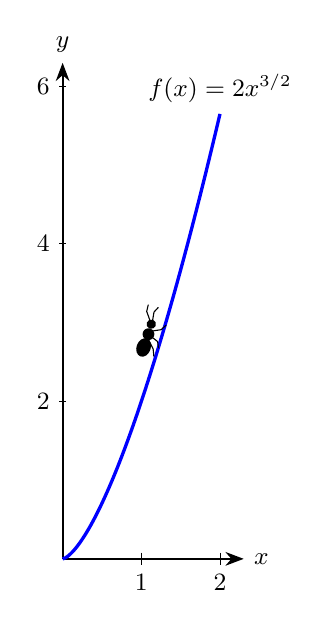
\begin{tikzpicture}[ x=1cm, y=1cm, >=Stealth, axis/.style={->, thick},
      curve/.style={blue, very thick}, every node/.style={font=\small} ]

      % Axes
      \draw[axis] (0,0) -- (2.3,0) node[right] {$x$}; \draw[axis] (0,0) --
      (0,6.3) node[above] {$y$};

      % Tick marks
      \foreach \x in {1,2} \draw (\x,0.08) -- (\x,-0.08) node[below] {$\x$};

      \foreach \y in {2,4,6} \draw (0.04,\y) -- (-0.04,\y) node[left] {$\y$};

      % Graph of f(x) = 2x^(3/2)
      \draw[curve, domain=0:2, samples=100, smooth] plot (\x,{2*\x*sqrt(\x)})
      node[above, black] {$f(x)=2x^{3/2}$};

      % Position of the ant
      \pgfmathsetmacro{\antx}{1.25}
      \pgfmathsetmacro{\anty}{2*\antx*sqrt(\antx)} \coordinate (ant) at
      (\antx,\anty);

      % Ant, rotated to approximately follow the tangent to the curve
      \begin{scope}[ shift={(ant)}, rotate=70, x=1.2cm, y=1cm, line cap=round,
        line join=round ]

        % Legs
        \draw[line width=0.4pt]
        (-0.05,0.15) -- (-0.13,0.05) -- (-0.20,0.01)
        (-0.01,0.14) -- (-0.04,0.03) -- (-0.10,-0.01)
        ( 0.04,0.15) -- ( 0.09,0.04) -- ( 0.15,0.00);

        % Body
        \fill (-0.15,0.17) ellipse[x radius=0.12cm,y radius=0.09cm]; \fill (
        0.00,0.17) circle[radius=0.075cm]; \fill ( 0.11,0.18)
        circle[radius=0.06cm];

        % Antennae
        \draw[line width=0.4pt] (0.14,0.21) -- (0.22,0.29) -- (0.29,0.30);
        \draw[line width=0.4pt] (0.15,0.18) -- (0.24,0.20) -- (0.30,0.17);
      \end{scope}
    \end{tikzpicture}
  \end{center}
  \textit{Solution:} $f'(x) = 3x^{\frac{1}{2}}$, so
  \begin{align*}
    (\text{Arc length})
    &= \int_{0}^{2} \sqrt{1+\left[ f'(x) \right]^{2} }dx\\
    &= \int_{0}^{2} \sqrt{1+9x }dx
  \end{align*}
  which we can solve with a $u$-substitution, taking $u=1+9x$. Doing this
  gives a length of about $6.06$. 
\end{example}



The \demph{hyperbolic cosine} and \demph{hyperbolic sine} functions are defined as
\begin{equation*}
  \demph{\cosh(x)} := \frac{e^{x}+e^{-x}}{2},  \qquad \demph{\sinh(x)} :=  \frac{e^{x}-e^{-x}}{2}.
\end{equation*}
These two functions are ``nice'' in that they behave in some respects
similarly to the standard sine and cosine functions; in particular, $\cosh$ is
an even function  (like $\cos(x)$) and $\sinh(x)$ is odd (like $\sin(x)$).

One can check they satisfy:
\begin{equation}\label{eq:hyperbolic derivatives}
  \cosh'(x) = \sinh(x), \qquad \sinh'(x)=\cosh(x).
\end{equation}
Also, we have the following identity:
\begin{equation}\label{eq:hyperbolic-square-identity}
  \cosh^{2}(x)- \sinh^{2}(x) =1.
\end{equation}
A hanging chain forms a curve known as a \demph{catenary}. The general
formula of a catenary is a function involving hyperbolic cosine; in the next
example, we'll consider the simplest case.


\begin{example}[Arc length]
  \label{ex:arc-length-sinh}


  % which has general equation
  % \begin{equation*}
  %   y = a\cosh \left( \frac{x-h}{a} \right)+k,
  % \end{equation*}
  % where $a>0$, $h$ and $k$ are physical parameters.

  Suppose $f(x)=\cosh(x)$ represents a chain from two endpoints at $x=-3$ and
  $x=3$. Find the length of the chain.

  \begin{center}
    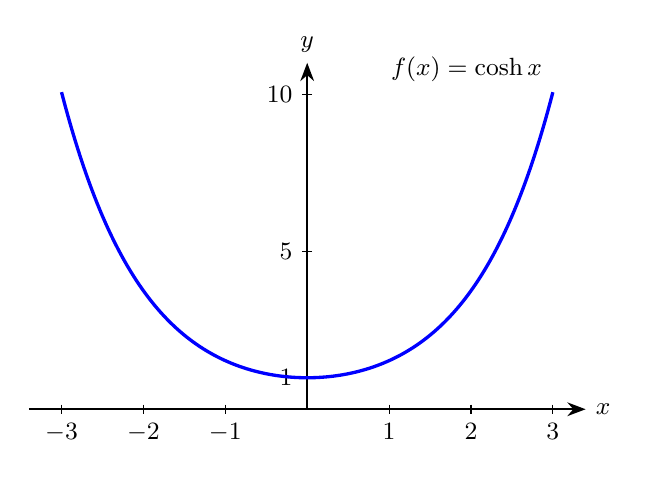
\begin{tikzpicture}[scale=.8, x=1.3cm, y=0.5cm, >=Stealth, axis/.style={->, thick},
      curve/.style={blue, very thick}, every node/.style={font=\small}]
      % Axes
      \draw[axis] (-3.4,0) -- (3.4,0) node[right] {$x$};
      \draw[axis] (0,0) -- (0,11) node[above] {$y$};
      % x-axis ticks
      \foreach \x in {-3,-2,-1,1,2,3} \draw (\x,0.15) -- (\x,-0.15) node[below] {$\x$};
      % y-axis ticks
      \foreach \y in {1,5,10} \draw (0.06,\y) -- (-0.06,\y) node[left] {$\y$};
      % Graph of f(x) = cosh(x)
      \draw[curve, domain=-3:3, samples=150, smooth]
      plot (\x,{(exp(\x)+exp(-1*(\x)))/2}) node[above left, black] {$f(x)=\cosh x$};
    \end{tikzpicture}


  \end{center}

  \begin{align*}
    (\text{length of chain}) 
    &= \int_{-3}^{3}\sqrt{1+ \left[\cosh'(x) \right]^{2} }dx\\
    &= \int_{-3}^{3}\sqrt{1+ \sinh^{2}(x) }dx &&\text{since $\cosh'(x)=\sinh(x)$ by \cref{eq:hyperbolic derivatives} }\\
    &= \int_{-3}^{3}\sqrt{\cosh^{2}(x) }dx &&\text{by \cref{eq:hyperbolic-square-identity} }\\
    &= \int_{-3}^{3}\cosh(x) dx &&\text{since $\cosh(x)>0$ for all $x\in \R$}\\
    &= \left[ \sinh(x) \right]_{x=-3}^{x=3}  &&\text{since $\sinh'(x)=\cosh(x)$ \cref{eq:hyperbolic derivatives}}\\
    &= \sinh(3) - \sinh(3)\\
    &\approx 20.036
\end{align*}


  
%   Find the length of the curve defined by $f(x) = \cosh(x) =\frac{1}{2} \left( e^{x}+e^{-x} \right)$
%   from $x=-1$ to $x=3$.

%   \textit{Solution:} We first claim that the following equality holds:
%   \begin{equation}\label{eq:1}
%     1+\left[ f'(x) \right]^{2}  = \left( \frac{e^{x}+e^{-x}}{2} \right)^{2}.
%   \end{equation}
%   This equality isn't obvious... it takes some work to deduce, which is shown below:
%   \begin{proof}[Proof of \cref{eq:1}]
%     Observe that $f'(x) = \frac{1}{2}(e^{x}-e^{-x})$. Therefore
%     \begin{align*}
%       1+\left[ f'(x) \right]^{2}
%       &= 1 + \left[ \frac{1}{2}\left( e^{x}-e^{-x} \right)  \right]^{2}\\ 
%       &= 1 + \frac{1}{4}\left( e^{2x} - 2 + e^{-2x} \right)\\ 
%       &= \frac{1}{4} e^{2x} + \frac{1}{2} + \frac{1}{4}e^{-2x}  &&\text{expanding everything out } \\ 
%       &= \frac{1}{4} \left( e^{2x}+2+e^{-2x} \right) &&\text{factor out $\frac{1}{4}$ }\\
%       &= \frac{1}{4}\left( e^{x}+e^{-x} \right)^{2}\\ 
%       &= \left( \frac{e^{x}+e^{-x}}{2} \right)^{2}. 
%     \end{align*}
%     This shows that \cref{eq:1} holds.
%   \end{proof}

%   Now with \cref{eq:1} in hand, everything simplifies really nicely when we apply the formula from
%   \cref{thm:arc-length-formula}:
%   \begin{align*}
%     \text{Arc Length} 
%     &= \int_{-1}^{3} \sqrt{1+\left[ f'(x) \right]^{2} }dx\\
%     &= \int_{-1}^{3} \sqrt{\left( \frac{e^{x}+e^{-x}}{2} \right)^{2}  }dx\\
%     &= \int_{-1}^{3} \frac{e^{x}+e^{-x}}{2}dx\\
%     &= \frac{1}{2}\int_{-1}^{3} \left( e^{x}+e^{-x} \right) dx\\
%     &= \frac{1}{2} \left[e^{x}-e^{-x} \right]_{x=-1}^{x=3}\\
%     &= \frac{1}{2} \left[ \left( e^{3} - e^{-3} \right)  - \left( e^{-1}-e^{1} \right)  \right]\\
%     &\approx 11.2
%   \end{align*}  
\end{example}

\Fl{Tips}
\begin{itemize}
  \item Check that your answer is positive. Arc length is never negative.
  \item These problems are usually contrived so that you can actually do the integral. If the integral
  looks took hard, double check your work. Also, there might be a trick to the integral. 
\end{itemize}

\end{document}